% Compilation : pdflatex F4.tex (deux fois).
% Document autonome : texte, formules et figures TikZ modifiables.
% Les reperes Source renvoient aux pages du manuscrit.
\documentclass[11pt,a4paper]{article}
\usepackage[utf8]{inputenc}
\usepackage[T1]{fontenc}
\usepackage[provide=*,french]{babel}
\usepackage[scaled=.95]{helvet}
\renewcommand{\familydefault}{\sfdefault}
\usepackage{amsmath,amssymb,esint,array,tabularx}
\usepackage{geometry}
\geometry{left=15mm,right=15mm,top=18mm,bottom=18mm,headheight=14pt,headsep=6mm}
\usepackage{fancyhdr,lastpage,tikz}
\usetikzlibrary{arrows.meta,calc,decorations.pathreplacing,decorations.pathmorphing,decorations.markings,patterns}
\usepackage[most]{tcolorbox}
\usepackage{enumitem,titlesec,needspace,hyperref}
\hypersetup{hidelinks,pdftitle={Dynamique des fluides parfaits},pdfsubject={Cours de physique}}
\pagestyle{fancy}\fancyhf{}
\fancyhead[L]{\small Physique F4 - Dynamique des fluides parfaits - inspiré par les cours de Mme Mesnil}
\fancyhead[R]{\small\thepage/\pageref{LastPage}}
\fancyfoot[R]{\small PC-PC*}
\renewcommand{\headrulewidth}{0pt}
\clubpenalty=10000\widowpenalty=10000\displaywidowpenalty=10000
\setlength{\parindent}{0pt}\setlength{\parskip}{4pt}
\setlength{\abovedisplayskip}{6pt}\setlength{\belowdisplayskip}{6pt}
\AtBeginEnvironment{center}{\setlength{\topsep}{4pt}\setlength{\partopsep}{0pt}}
\setlist[itemize]{leftmargin=5mm,itemsep=3pt,topsep=3pt,label=\(\rightarrow\)}
\setlist[enumerate]{leftmargin=6mm,itemsep=3pt,topsep=3pt}
\renewcommand{\thesection}{\Roman{section}}
\renewcommand{\thesubsection}{\thesection.\arabic{subsection}}
\titleformat{\section}{\Large\bfseries}{\thesection.}{.4em}{}
\titleformat{\subsection}{\large\bfseries}{\thesubsection.}{.4em}{}[\titlerule]
\titleformat{\subsubsection}{\normalsize\bfseries}{\alph{subsubsection})}{.5em}{}
\titlespacing*{\section}{0pt}{11pt}{6pt}
\titlespacing*{\subsection}{0pt}{9pt}{5pt}
\titlespacing*{\subsubsection}{0pt}{8pt}{4pt}
\newtcolorbox{cadre}[1][]{enhanced,sharp corners,colback=white,colframe=black,boxrule=1.1pt,left=7pt,right=7pt,top=5pt,bottom=5pt,before skip=7pt,after skip=7pt,#1}
\newtcolorbox{exemple}[1][]{enhanced,sharp corners,colback=white,colframe=black,boxrule=.7pt,left=8pt,right=8pt,top=6pt,bottom=6pt,before skip=8pt,after skip=8pt,#1}
\tcbset{etoiles/.style={width=\dimexpr\linewidth-22mm\relax,overlay={\node[anchor=west,inner sep=0pt,font=\small] at ([xshift=2mm]frame.east) {\(#1\)};}}}
\newcommand{\dd}{\mathrm d}
\newcommand{\vv}{\vec v}
\newcommand{\grad}{\overrightarrow{\mathrm{grad}}}
\newcommand{\pd}[2]{\frac{\partial #1}{\partial #2}}
\newcommand{\ux}{\vec u_x}\newcommand{\uy}{\vec u_y}\newcommand{\uz}{\vec u_z}
\newcommand{\cste}{\mathrm{cste}}
\newcommand{\titr}[1]{\par\textbf{\underline{#1}}\par\nopagebreak[3]}
\newcommand{\planpart}[2]{\par\vspace{5pt}{\bfseries #1. #2}\par}
\newcommand{\plansub}[2]{\hspace*{7mm}{\itshape #1) #2}\par}
\newcommand{\plansubsub}[1]{\hspace*{15mm}{\itshape #1}\par}
\tikzset{>=Stealth,every node/.style={font=\small},flow/.style={thick,->},edge/.style={thick}}
\newcommand{\etoiles}[1]{\foreach \i in {1,...,#1}{\mathord{\star}\,}}
\newcommand{\R}{\mathcal R}
\newcommand{\Dv}{\frac{\mathrm D\vec v}{\mathrm Dt}}
\newcommand{\conv}{(\vec v\cdot\grad)\vec v}
\newcommand{\fv}{\vec f_v}\newcommand{\fvt}{\vec f_{v,\mathrm{tot}}}\newcommand{\fvi}{\vec f_{v,\mathrm{inertie}}}
\newcommand{\diver}{\operatorname{div}}
\newcommand{\Rey}{R_e}
\newcommand{\rot}{\overrightarrow{\mathrm{rot}}}
\newcommand{\epv}{E_{pV}}
\tikzset{courant/.style={blue!65!black,thick,postaction={decorate},decoration={markings,mark=at position .55 with {\arrow{Stealth}}}},force/.style={red!65!black,thick,->},pression/.style={violet!80!black}}
% Figures reutilisees, entierement editables.
\newcommand{\coanda}[2]{\begin{tikzpicture}[scale=.85]
\ifnum#1=0
\draw[thick] (0,0) circle(.36);\fill (1.3,2) circle(1.6pt);\draw (0,0)--(1.3,2);\draw[dashed] (1.3,2)--(1.3,.15);
\draw (1.3,1.35) arc(-90:-123:.65);\node at (.95,1.03){$\theta$};
\draw[blue!65!black,thick] (-.5,2.1)--(-.5,.3)..controls(-.5,-.6)and(.2,-1)..(.7,-1.3);
\draw[blue!65!black,thick] (-.36,2.1)--(-.36,.4)..controls(-.35,-.55)and(.4,-.8)..(.85,-1.05);
\draw[blue!65!black,thick,->] (-.5,1.85)--(-.5,1.3);\draw[blue!65!black,thick,->] (-.36,1.35)--(-.36,.85);\node[left] at (-.65,1){Eau};
\ifnum#2=1
\draw[force] (0,0)--(0,-1.7) node[below]{$m\vec g$};\draw[force] (0,0)--(-1.2,-.75) node[below left,align=center]{$\vec F_{\mathrm{pression}}$};
\node[pression,left] at (-.75,.2){$P_0$};\node[pression,right] at (.5,.05){$P_0$};\node[pression,right] (pwater) at (.9,-1.15){$P_1$};\draw[pression,->] (pwater.west)--(.15,-.7);\node[pression] at (1.15,-1.85){$P_1<P_0$};
\fi
\else
\draw[thick] (0,0) circle(.45);
\draw[blue!65!black,thick] (-1.9,-.15)..controls(-.8,1.3)and(.25,1.25)..(1.4,.25);
\draw[blue!65!black,thick] (-1.65,-.35)..controls(-.7,.95)and(.2,.9)..(1.25,.05);
\draw[blue!65!black,thick,->] (-1.7,.1)--(-1.38,.4);\draw[blue!65!black,thick,->] (-1.4,-.05)--(-1.1,.22);\node[left] at (-1.7,-.45){Air};
\ifnum#2=1
\draw[force] (0,0)--(0,-1.5) node[right]{$m\vec g$};\draw[force] (0,0)--(-.25,1.65) node[above]{$\vec F_{\mathrm{pression}}$};
\node[pression] at (-1.2,.85){$P_0$};\node[pression] at (.85,1.05){$P_0$};\node[pression,right] (pair) at (1.3,-.65){$P_1$};\draw[pression,->] (pair.north west)--(.55,.55);\node[pression,left] at (-.45,-.25){$P_0$};
\fi\fi\end{tikzpicture}}
\newcommand{\feuille}[1]{\begin{tikzpicture}[scale=.8]
\draw[thick] (0,.1)..controls(1.6,.3)and(2.1,-.4)..(2.7,-1.2);
\foreach \y in {.55,.8,1.05}{\draw[courant] (-1,\y)--(.8,\y);}\node[above] at (-.3,1.1){Souffle};
\ifnum#1=0\draw[dashed] (0,.1)..controls(1.2,.1)and(2,.4)..(2.7,.7);\draw[force] (2,-.65)--(2.25,.65);\node[right] at (2.6,-.7){Feuille};\node[pression] at (.6,-.5){$P_0$};
\else\fill (0,.6) circle(1.5pt) node[below left]{$A$};\fill (1.5,.25) circle(1.5pt) node[below left]{$B$};\node[pression,left] at (-1.15,.6){$P_0$};\node[pression,right] at (1.9,.65){$P_B$};\node[pression] at (.8,-.45){$P_0$};\draw[force] (1.45,-.15)--(1.6,.9);\fi
\end{tikzpicture}}
\newcommand{\entonnoir}[1]{\begin{tikzpicture}[scale=.85]
\draw[thick] (-.3,2)--(-.3,.7)--(-1.9,-.9) (.3,2)--(.3,.7)--(1.9,-.9);
\draw[thick] (0,0) circle(.55);
\draw[blue!65!black,thick] (-.12,1.85)--(-.12,.8)..controls(-.2,.65)and(-.6,.35)..(-1.45,-.55);
\draw[blue!65!black,thick] (.12,1.85)--(.12,.8)..controls(.2,.65)and(.6,.35)..(1.45,-.55);
\draw[blue!65!black,thick,->] (-.12,1.8)--(-.12,1.4);\draw[blue!65!black,thick,->] (.12,1.3)--(.12,.9);\node[pression] at (0,-1.1){$P_0$};
\ifnum#1=1\fill (0,2.1) circle(1.4pt) node[above left]{$A$};\node[pression,right] at (.3,2){$P_0$};\fill (-.62,.24) circle(1.4pt) node[below left]{$B$};\node[pression,left] at (-1.15,.05){$P_B$};\draw[force] (-.2,-.1)--(-1.2,.8) node[left]{$\vec F_{\mathrm{pression}}$};\draw[force] (.2,-.1)--(1.2,.8) node[right]{$\vec F_{\mathrm{pression}}$};\fi
\end{tikzpicture}}
\newcommand{\canettes}[1]{\begin{tikzpicture}[scale=.75]
\ifnum#1=0
\draw[thick] (-1,0) rectangle(-.4,1.4);\draw[thick] (.4,0) rectangle(1,1.4);
\draw (-1.4,-.4)--(1.4,-.4);\foreach\x in{-1,-.6,-.2,.2,.6,1}{\draw (\x,-.2) circle(.12);}
\draw[force] (-.7,.7)--(-.05,.7);\draw[force] (.7,.7)--(.05,.7);
\else
\draw[thick] (-.8,.8) circle(.5);\draw[thick] (.8,.8) circle(.5);
\draw[courant] (-.7,-1.3)..controls(-.7,-.2)and(-.2,.3)..(-.18,.85);\draw[courant] (.7,-1.3)..controls(.7,-.2)and(.2,.3)..(.18,.85);
\fill (-.7,-1) circle(1.5pt) node[left]{$A$};\fill (0,.8) circle(1.5pt) node[above]{$B$};
\node[pression] at (-1.65,.8){$P_0$};\node[pression] at (1.65,.8){$P_0$};\node[pression] at (0,.3){$P_B$};\draw[force] (-.8,.8)--(-.1,.8);\draw[force] (.8,.8)--(.1,.8);
\fi\end{tikzpicture}}
\newcommand{\feuilleosc}[1]{\begin{tikzpicture}[scale=.75]
\draw[thick] (-1.7,0)--(2.4,0);\draw[thick] (-.9,2)..controls(-.7,1)and(.7,.15)..(1.9,0);
\foreach\y in{.4,.75,1.1}{\draw[courant] (-1.4,\y)--(.2,{\y*.4});}
\ifnum#1=0\node[above] at (-.5,1.9){Feuille};\node[left] at (-1.4,.8){Souffle};\draw[red!70!black,domain=.6:1.6,samples=50] plot(\x,{.2*sin(720*\x)});\node[below] at (1.2,-.3){Oscillations};
\else\fill (-1.1,.8) circle(1.4pt) node[above left]{$A$};\fill (.65,.15) circle(1.4pt) node[above right]{$B$};\node[pression] at (-1.65,1.4){$P_0$};\node[pression] at (1.4,1.5){$P_0$};\node[pression] at (1,-.5){$P_B$};\draw[force] (.65,.15)--(.1,-1.05);\fi
\end{tikzpicture}}
\newcommand{\venturi}{\draw[thick] (0,1)--(1.5,1)--(2.7,.3)--(4,.3)--(5.2,1)--(6.8,1);\draw[thick] (0,-1)--(1.5,-1)--(2.7,-.3)--(4,-.3)--(5.2,-1)--(6.8,-1);}
\newcommand{\cylindre}[1]{\begin{tikzpicture}[scale=.85]
\draw[->] (-3,0)--(3.5,0) node[right]{$x$};\draw[->] (0,-1.5)--(0,1.7) node[above]{$y$};\draw[thick] (0,0) circle(1);
\foreach\sgn in{-1,1}{\foreach\h in{.45,.8}{\draw[courant] (-3,\sgn*\h)..controls(-1.2,\sgn*\h)and(-1.4,{\sgn*(1.07+.4*\h)})..(0,{\sgn*(.97+.4*\h)})..controls(1.4,{\sgn*(1.07+.4*\h)})and(1.2,\sgn*\h)..(3,\sgn*\h);}}
\draw[courant] (-3,0)--(-1.1,0);\draw[courant] (1.1,0)--(3,0);\node at (.3,.25){$\Sigma$};
\ifnum#1=0\draw[force] (-.7,.7)--(-1.2,1.2) node[above left]{$\dd^2\vec S$};
\else\foreach\a in{45,135,225,315}{\draw[pression,->] (\a:1)--(\a:.4);}\node[pression,right] at (1.4,-1.3){$\dd^2\vec F_p$};\fi
\end{tikzpicture}}
\begin{document}
{\raggedright\fontsize{27}{31}\selectfont\bfseries Dynamique des fluides parfaits\par}
\vspace{4mm}
\begingroup\setlength{\parskip}{.7pt}
\planpart{I}{Équation d'Euler}
\plansub{1}{Équation d'Euler}
\plansub{2}{Quelques commentaires}
\plansub{3}{Influence de la courbure des lignes de champ sur la pression}
\plansubsub{a) Lignes de courant courbées}
\plansubsub{b) Lignes de courant parallèles}
\planpart{II}{Théorèmes de Bernoulli}
\plansub{1}{Mises en évidence expérimentales}
\plansub{2}{Fluide incompressible dans un écoulement stationnaire et irrotationnel}
\plansub{3}{Écoulement stationnaire, incompressible et homogène}
\plansub{4}{Fluide incompressible dans un écoulement irrotationnel}
\planpart{III}{Applications du théorème de Bernoulli}
\plansub{1}{Effet Venturi}
\plansub{2}{Tube de Pitot}
\plansub{3}{Vidange d'un réservoir}
\plansub{4}{Portance et effet Magnus}
\endgroup
% Source 1
\begin{itemize}
\item La dynamique consiste à déterminer le champ des vitesses à partir des forces.
\item Pour un fluide parfait, tout phénomène de diffusion est négligé. En particulier, la viscosité est négligée : $\eta=0$.
\item Le modèle du fluide parfait est valable pour un grand nombre de Reynolds. Pour l'air, cette approximation est souvent justifiée.
\item Dans la couche limite, proche des obstacles, le modèle du fluide parfait n'est pas valable.
\end{itemize}
\section{Équation d'Euler}
\subsection{Équation d'Euler}
\begin{center}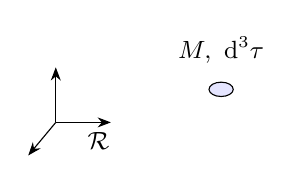
\begin{tikzpicture}[scale=.7]
\draw[->] (0,0)--(1,0);\draw[->] (0,0)--(0,1);\draw[->] (0,0)--(-.5,-.6);\node[below right] at (.4,0){$\R$};\draw[fill=blue!10] (3,.6) ellipse(.22 and .13);\node[above] at (3,.9){$M,\ \dd^3\tau$};
\end{tikzpicture}\end{center}
% Source 2
Le théorème de la quantité de mouvement appliqué à la particule fluide dans $\R$ donne
\[\mu\dd^3\tau\Dv=\underbrace{\fv}_{\substack{\text{équivalent volumique}\\\text{des forces à distance}}}\dd^3\tau-\grad P\,\dd^3\tau+\fvi\,\dd^3\tau.\]
\begin{cadre}[etoiles={\etoiles{5}}]\[\mu\Dv=\fvt-\grad P.\]\end{cadre}
\begin{cadre}[etoiles={\etoiles{5}}]\[\mu\left[\pd{\vec v}t+\conv\right]=\fvt-\grad P.\]\end{cadre}
Le terme $(\vec v\cdot\grad)\vec v$ n'est jamais négligeable pour un fluide parfait.
\begin{cadre}[etoiles={\etoiles{6}}]\[\mu\left[\pd{\vec v}t+\frac12\grad v^2+\rot\vec v\wedge\vec v\right]=\fvt-\grad P.\]\textbf{Équation d'Euler.}\end{cadre}
% Sources 3-4
\subsection{Quelques commentaires}
\begin{enumerate}
\item L'équation est non linéaire à cause du terme $(\vec v\cdot\grad)\vec v$ : c'est un enjeu de la dynamique des fluides parfaits.
\item L'équation d'Euler relie $\vec v$ et $P$. En mécanique des fluides, $\vec v(M,t)$ représente trois inconnues et $P(M,t)$ une inconnue.

\textbf{Fluide incompressible :} $\mu=\cste$ est connue. On a quatre inconnues et quatre équations : les trois composantes de l'équation d'Euler et $\diver\vec v=0$.

\textbf{Écoulement compressible :} $\mu(M,t)$ est inconnue. On a cinq inconnues et cinq équations : les trois composantes de l'équation d'Euler, la conservation de la masse
\[\pd\mu t+\diver(\mu\vec v)=0,\]
et une équation thermodynamique reliant $\mu$ et $P$. C'est le cas des ondes sonores.
\item Si $\|\conv\|\ll\|\partial\vec v/\partial t\|$, on peut linéariser l'équation d'Euler. C'est le cas pour les ondes sonores.
\item La plupart du temps, $\R$ est galiléen et $\fv=\mu\vec g$. L'équation d'Euler s'écrit
\begin{cadre}\[\mu\Dv=\mu\vec g-\grad P.\]\end{cadre}
En statique, $\vec v=\vec0$, donc $\mu\vec g=\grad P$.
\end{enumerate}
\subsection{Influence de la courbure des lignes de champ sur la pression}
% Sources 4-5
Dans la suite du cours, $\R$ est galiléen : il n'y a pas de forces d'inertie et $\fvt=\fv$. Il faut adapter les résultats dans les exercices où $\R$ est non galiléen.
\begin{cadre}\[\mu\Dv=\fv-\grad P.\]\end{cadre}
Cette équation relie $\vec v(M,t)$ et $P(M,t)$. On cherche le lien entre la direction de $\vec v$ et son influence sur $P$.
\subsubsection{Lignes de courant courbées}
\begin{center}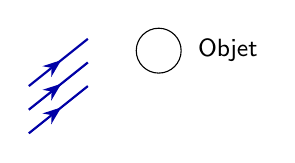
\begin{tikzpicture}[scale=.75]
\draw (2,1) circle(.38);\node[right] at (2.5,1){Objet};\foreach\y in{-.4,0,.4}{\draw[courant] (-.2,\y)--(.8,{\y+.8});}
\end{tikzpicture}\end{center}
L'écoulement est dévié par l'objet.
\titr{Effet Coanda}
\begin{center}\begin{minipage}{.47\linewidth}\centering\coanda{0}{0}\par Le jet d'eau est dévié par la balle. La balle est « aspirée » par le jet d'eau.\end{minipage}\hfill\begin{minipage}{.47\linewidth}\centering\coanda{1}{0}\par Le jet d'air maintient la balle.\end{minipage}\end{center}
% Source 6
\[\mu\Dv=\fv-\grad P.\]
\textbf{Hypothèse :} $\|\fv\|\ll\|\grad P\|$. Cette hypothèse est valable pour l'air et, pour l'eau, sur de petits jets.
\begin{center}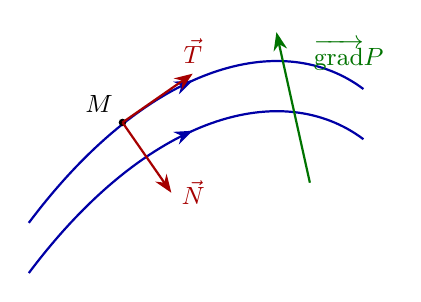
\begin{tikzpicture}[scale=.85]
\draw[courant] (-2,-.8)..controls(-.2,1.6)and(1.8,2.1)..(3,1.2);\draw[courant] (-2,-1.55)..controls(-.2,.85)and(1.8,1.35)..(3,.45);
\fill (-.6,.7) circle(1.6pt) node[above left]{$M$};\draw[force] (-.6,.7)--(.45,1.43) node[above]{$\vec T$};\draw[force] (-.6,.7)--(.13,-.35) node[right]{$\vec N$};\draw[->,green!45!black,thick] (2.2,-.2)--(1.7,2.05) node[right=8pt,pos=.85]{$\grad P$};
\end{tikzpicture}\end{center}
\[\vec v(M,t)=v(M,t)\vec T.\]
$(\vec T,\vec N)$ est la base de Frenet ; $\vec N$ est dirigé vers le centre de courbure. On admet que
\[\Dv=\frac{\mathrm Dv}{\mathrm Dt}\vec T+\frac{v^2}{R}\vec N.\]
% Source 7
L'équation d'Euler donne
\[\mu\Dv=-\grad P=\mu\frac{\mathrm Dv}{\mathrm Dt}\vec T+\mu\frac{v^2}{R}\vec N.\]
\begin{cadre}\[-(\grad P)\cdot\vec N=\mu\frac{v^2}{R}>0.\]\end{cadre}
Ainsi, $\grad P\cdot\vec N<0$.
\begin{cadre}[etoiles={\etoiles{3}}]
Dans un écoulement de fluide parfait où les forces à distance sont négligeables devant les forces de pression, la pression augmente quand on s'éloigne du centre de courbure.
\end{cadre}
\begin{center}\begin{minipage}{.49\linewidth}\centering\coanda{0}{1}\end{minipage}\hfill\begin{minipage}{.49\linewidth}\centering\coanda{1}{1}\par $P_1<P_0$.\end{minipage}\end{center}
% Source 8
\subsubsection{Lignes de courant parallèles}
\begin{center}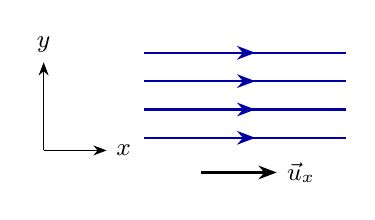
\begin{tikzpicture}[scale=.8]
\draw[->] (-1,0)--(0,0) node[right]{$x$};\draw[->] (-1,0)--(-1,1.4) node[above]{$y$};\foreach\y in{.2,.65,1.1,1.55}{\draw[courant] (.6,\y)--(3.8,\y);}\draw[->,thick] (1.5,-.35)--(2.7,-.35) node[right]{$\ux$};
\end{tikzpicture}\end{center}
\[\vec v(M,t)=v_x(M,t)\ux,\qquad\mu\Dv=\fv-\grad P,\]
\[\Dv=\pd{v_x}t\ux+\left(v_x\pd{v_x(M,t)}x\right)\ux.\]
Prenons $\vec u\perp\ux$, par exemple $\uy$ ou $\uz$ :
\[\mu\Dv\cdot\vec u=0=(\fv-\grad P)\cdot\vec u.\]
\begin{cadre}[etoiles={\etoiles{5}}]
Dans un écoulement parfait dont les lignes de courant sont parallèles à une direction fixe, la répartition de la pression dans une direction perpendiculaire aux lignes de courant est hydrostatique.
\end{cadre}
% Source 9
\textbf{Remarque :} si l'écoulement n'est pas parfait, on ajoute $\eta\Delta\vec v$. Ce terme est toujours parallèle à $\ux$, donc $\eta\Delta\vec v\cdot\vec u=0$. La propriété est donc valable aussi pour des écoulements non parfaits.
\begin{exemple}[breakable,etoiles={\etoiles{5}}]
\textbf{Écoulement d'un fleuve}
\begin{center}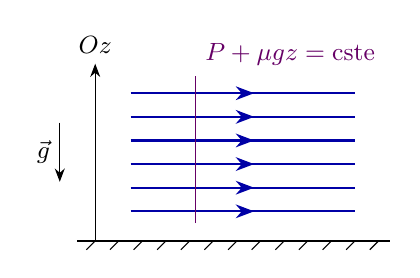
\begin{tikzpicture}[scale=.75]
\draw[->] (0,0)--(0,3) node[above]{$Oz$};\draw[thick] (-.3,0)--(5,0);\foreach\x in{0,.4,...,4.8}{\draw (\x,0)--++(-.15,-.15);}\foreach\y in{.5,.9,1.3,1.7,2.1,2.5}{\draw[courant] (.6,\y)--(4.4,\y);}\draw[pression] (1.7,.3)--(1.7,2.8) node[above right]{$P+\mu gz=\cste$};\draw[->] (-.6,2)--(-.6,1) node[midway,left]{$\vec g$};
\end{tikzpicture}\end{center}
\[P(z)=P_0-\mu gz,\qquad\text{comme en statique.}\]
\end{exemple}
\begin{exemple}[breakable,etoiles={\etoiles{4}}]
\textbf{Jet libre}
\begin{center}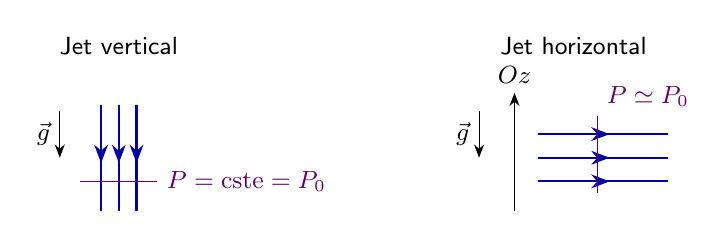
\begin{tikzpicture}[scale=.75]
\node at (0,2.5){Jet vertical};\foreach\x in{-.3,0,.3}{\draw[courant] (\x,1.5)--(\x,-.3);}\draw[pression] (-.65,.2)--(.65,.2) node[right]{$P=\cste=P_0$};\draw[->] (-1,1.4)--(-1,.6) node[midway,left]{$\vec g$};
\begin{scope}[xshift=6.7cm]\node at (1,2.5){Jet horizontal};\draw[->] (0,-.3)--(0,1.7) node[above]{$Oz$};\foreach\y in{.2,.6,1}{\draw[courant] (.4,\y)--(2.6,\y);}\draw[pression] (1.4,0)--(1.4,1.3) node[above right]{$P\simeq P_0$};\draw[->] (-.6,1.4)--(-.6,.6) node[midway,left]{$\vec g$};\end{scope}
\end{tikzpicture}\end{center}
Pour le jet horizontal, dans l'air, $P=P_0$. Dans l'eau, si la section est petite, on néglige le poids et $P=P_0$.
% Source 10
\textbf{Exemple :}
\begin{center}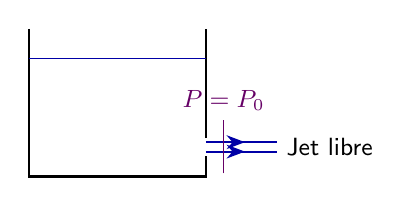
\begin{tikzpicture}[scale=.75]
\draw[thick] (0,2.5)--(0,0)--(3,0)--(3,.35) (3,.65)--(3,2.5);\draw[blue!65!black] (0,2)--(3,2);\draw[courant] (3,.42)--(4.2,.42);\draw[courant] (3,.58)--(4.2,.58);\draw[pression] (3.3,.05)--(3.3,.95) node[above]{$P=P_0$};\node[right] at (4.2,.5){Jet libre};
\end{tikzpicture}\end{center}
\end{exemple}
\section{Théorèmes de Bernoulli}
\subsection{Mises en évidence expérimentales}
% Sources 10-11
\begin{exemple}
\textbf{Expérience 1}
\begin{center}\feuille{0}\end{center}
La feuille est aspirée vers le haut. La vitesse est associée à une chute de pression.
\end{exemple}
\begin{exemple}
\textbf{Expérience 2}
\begin{center}\entonnoir{0}\end{center}
Souffler dans l'entonnoir permet de tenir la balle dans l'entonnoir. Le souffle semble aspirer la balle.
\end{exemple}
\begin{exemple}
\textbf{Expérience 3}
\begin{center}\canettes{0}\end{center}
Souffler entre deux canettes les met en mouvement et provoque leur collision.
\end{exemple}
\begin{exemple}
\textbf{Expérience 4}
\begin{center}\feuilleosc{0}\end{center}
Un souffle seul met la feuille en oscillation.
\end{exemple}
\begin{exemple}
\textbf{Expérience 5}
\begin{center}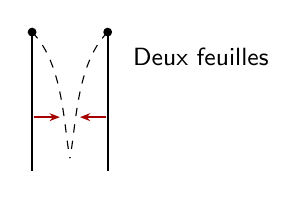
\begin{tikzpicture}[scale=.8]
\fill (-.6,2) circle(2pt);\fill (.6,2) circle(2pt);\draw[thick] (-.6,2)--(-.6,-.2) (.6,2)--(.6,-.2);\draw[dashed] (-.6,2)..controls(-.1,1.5)and(-.1,.5)..(0,0);\draw[dashed] (.6,2)..controls(.1,1.5)and(.1,.5)..(0,0);\node[right] at (.85,1.6){Deux feuilles};\draw[red!65!black,thick,-{Stealth[length=1.3mm,width=1mm]}] (-.57,.65)--(-.16,.65);\draw[red!65!black,thick,-{Stealth[length=1.3mm,width=1mm]}] (.57,.65)--(.16,.65);
\end{tikzpicture}\end{center}
Souffler entre deux feuilles les colle.
\end{exemple}
\subsection{Fluide incompressible dans un écoulement stationnaire et irrotationnel}
Cette version du théorème n'est pas au programme.
% Source 12
\begin{align*}
\mu\Dv&=\fv-\grad P\\
&=\mu\left[\pd{\vec v}t+\conv\right]\\
&=\mu\left[\pd{\vec v}t+\frac12\grad v^2+\rot\vec v\wedge\vec v\right].
\end{align*}
Dans la suite du cours, on suppose que toutes les forces à distance sont \textbf{conservatives}.
\begin{cadre}\[\fv=-\grad\epv.\]\end{cadre}
$\fv$ est la densité volumique de force et $\epv$ l'énergie potentielle volumique. Unité de $\epv$ : $\mathrm{J\,m^{-3}}$.
\begin{exemple}\textbf{Exemple :}\[\fv=\mu\vec g\quad\Longrightarrow\quad\epv=\mu gz+\cste.\]\end{exemple}
\[\mu\left[\pd{\vec v}t+\frac12\grad v^2+\rot\vec v\wedge\vec v\right]=-\grad(P+\epv).\]
\titr{Hypothèses}
\begin{itemize}
\item L'écoulement est stationnaire : $\partial\vec v/\partial t=\vec0$.
\item L'écoulement est irrotationnel : $\rot\vec v=\vec0$.
\item L'écoulement est incompressible : $\mu=\cste$.
\end{itemize}
% Source 13
Ainsi,
\[\grad\left(\frac12\mu v^2\right)=-\grad(P+\epv),\qquad\grad\left(P+\epv+\frac12\mu v^2\right)=\vec0.\]
\begin{cadre}[etoiles={\etoiles{5}}]\[P+\epv+\frac12\mu v^2=\cste\]\nobreak dans tout l'écoulement.\end{cadre}
\begin{cadre}[etoiles={\etoiles{4}}]
Dans un écoulement parfait, stationnaire, irrotationnel et incompressible, la quantité $P+\epv+\frac12\mu v^2$ est constante dans tout l'écoulement.
\end{cadre}
\textbf{Remarque :} si $\epv=\mu gz$,
\[P+\frac12\mu v^2+\mu gz=\cste.\]
Cette quantité est la « charge de l'écoulement ».
\titr{Hypothèses dans la pratique}
\begin{itemize}
\item Stationnaire : il s'agit du régime permanent.
\item Incompressible : cette hypothèse convient aux expériences où $v\ll c_{\mathrm{son}}$.
\item Irrotationnel : c'est une hypothèse forte et contraignante.
\end{itemize}
% Source 14
\subsection{Écoulement stationnaire, incompressible et homogène}
\textbf{Remarque :} c'est la seule version du théorème au programme.
\[\mu\left[\pd{\vec v}t+\frac12\grad v^2+\rot\vec v\wedge\vec v\right]=-\grad(P+\epv).\]
L'écoulement est stationnaire : $\partial\vec v/\partial t=\vec0$. Les trajectoires coïncident avec les lignes de courant.

L'écoulement est incompressible : $\mu$ est constante sur une trajectoire, donc sur une ligne de courant.
\begin{center}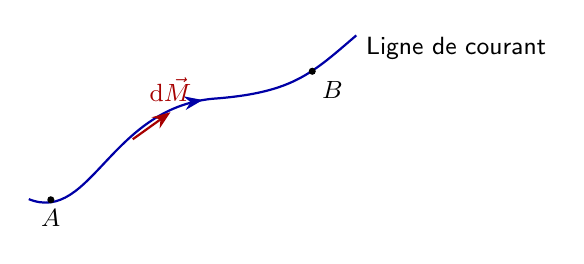
\begin{tikzpicture}[scale=.8]
\draw[courant] (0,0)..controls(1,-.4)and(1.3,1.5)..(3,1.6)..controls(4.2,1.7)and(4.5,2)..(5.2,2.6);
\fill (.35,-.01) circle(1.6pt) node[below]{$A$};\fill (4.5,2.03) circle(1.6pt) node[below right]{$B$};\draw[force] (1.65,.95)--(2.25,1.38) node[above]{$\dd\vec M$};\node[right] at (5.2,2.4){Ligne de courant};
\end{tikzpicture}\end{center}
% Source 15
\begin{align*}
\int_A^B\left(\frac\mu2\grad v^2+\mu\rot\vec v\wedge\vec v\right)\cdot\underbrace{\dd\vec M}_{\parallel\vec v}
&=\int_A^B-\grad(P+\epv)\cdot\dd\vec M,\\[4pt]
\int_A^B\left(\frac\mu2\grad v^2+\grad(P+\epv)\right)\cdot\dd\vec M&=0,\\[4pt]
\int_A^B\underbrace{\grad\left(\frac12\mu v^2+P+\epv\right)\cdot\dd\vec M}_{\dd(P+\epv+\frac12\mu v^2)}&=0.
\end{align*}
\begin{cadre}[etoiles={\etoiles{5}}]\[P(A)+\frac12\mu v^2(A)+\epv(A)=P(B)+\frac12\mu v^2(B)+\epv(B).\]\end{cadre}
\begin{cadre}
Dans un écoulement parfait, stationnaire, incompressible et homogène, la quantité $P+\epv+\frac12\mu v^2$ est constante sur une ligne de courant.
\end{cadre}
\textbf{Remarque :} selon les livres, « homogène » peut signifier :
\begin{itemize}
\item Définition 1 : il s'agit du même fluide en écoulement partout.
\item Définition 2 : $\mu$ est indépendante du point $M$. Cette hypothèse est incluse dans l'hypothèse d'incompressibilité.
\end{itemize}
% Source 16
\begin{exemple}
\textbf{Expérience 1}
\begin{center}\feuille{1}\end{center}
\[P_0+\frac12\mu v_A^2=P_B+\frac12\mu v_B^2.\]
Le resserrement des lignes de courant donne $v_B>v_A$, donc $P_B<P_A$.
Le même phénomène se produit pour les toits pendant une tempête.
\begin{center}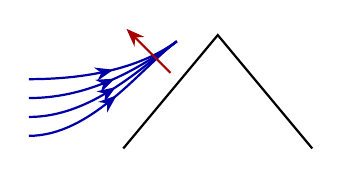
\begin{tikzpicture}[scale=.8]
\draw[thick] (0,0)--(1.5,1.8)--(3,0);\foreach\y in{.2,.5,.8,1.1}{\draw[courant] (-1.5,\y)..controls(-.5,\y)and(.3,1.3)..(.85,1.7);}\draw[force] (.75,1.2)--(.05,1.9);
\end{tikzpicture}\end{center}
\end{exemple}
\begin{exemple}
\textbf{Expérience 2}
\begin{center}\entonnoir{1}\end{center}
\[P_A=P_0,\qquad P_0+\frac12\mu v_A^2=P_B+\frac12\mu v_B^2.\]
Le resserrement des lignes de courant donne $v_B>v_A$, donc $P_B<P_0$.
\end{exemple}
% Source 17
\begin{exemple}
\textbf{Expérience 3}
\begin{center}\canettes{1}\end{center}
\[P_B<P_0.\]
\end{exemple}
\begin{exemple}
\textbf{Expérience 4}
\begin{center}\feuilleosc{1}\end{center}
\[P_B<P_0=P_A.\]
Après que la feuille a été collée à la table, une accumulation d'air la soulève à nouveau, d'où les oscillations.
\end{exemple}
\subsection{Fluide incompressible dans un écoulement irrotationnel}
% Sources 17-18
\[\mu\pd{\vec v}t+\frac\mu2\grad v^2+\underbrace{\mu\rot\vec v\wedge\vec v}_{\vec0}=-\grad(P+\epv),\]
\[\mu\pd{\vec v}t+\grad\left(\frac12\mu v^2+P+\epv\right)=\vec0.\]
L'écoulement est irrotationnel : il existe $\Phi$ tel que $\vec v=\grad\Phi$.
\[\mu\frac\partial{\partial t}\grad\Phi+\grad\left(\frac12\mu v^2+P+\epv\right)=\vec0,\]
\[\grad\left[\mu\pd\Phi t+\frac12\mu v^2+P+\epv\right]=\vec0.\]
\begin{cadre}[etoiles={\etoiles{2}}]\[\mu\pd\Phi t+\frac12\mu v^2+P+\epv=f(t)\]\nobreak dans tout l'écoulement.\end{cadre}
Dans un écoulement parfait, irrotationnel et incompressible, $\mu\partial\Phi/\partial t+\frac12\mu v^2+P+\epv$ est une fonction du temps.
\section{Applications du théorème de Bernoulli}
% Sources 18-19
Dans toute cette partie, on se place dans le cas exigible au programme : l'écoulement est parfait, stationnaire, incompressible et homogène.
\subsection{Effet Venturi}
S'il y a un resserrement des lignes de courant, la vitesse augmente et la pression diminue. Cela concerne toutes les expériences précédentes.
\begin{center}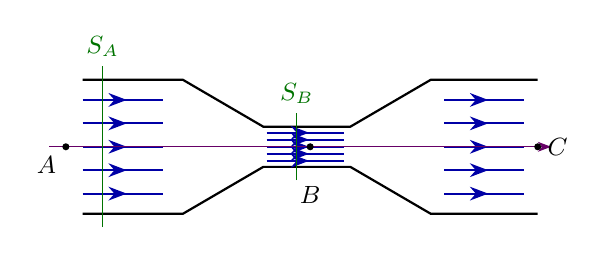
\begin{tikzpicture}[scale=.85]
\venturi
\foreach\y in{-.7,-.35,0,.35,.7}{\draw[courant] (0,\y)--(1.2,\y);\draw[courant] (2.75,{\y*.3})--(3.9,{\y*.3});\draw[courant] (5.4,\y)--(6.6,\y);}
\draw[pression,->] (-.5,0)--(7,0);\fill(-.25,0)circle(1.5pt)node[below left]{$A$};\fill(3.4,0)circle(1.5pt);\node[below] at (3.4,-.45){$B$};\fill(6.8,0)circle(1.5pt)node[right]{$C$};
\draw[green!45!black] (.3,-1.2)--(.3,1.2) node[above]{$S_A$};\draw[green!45!black] (3.2,-.5)--(3.2,.5) node[above]{$S_B$};
\end{tikzpicture}\end{center}
On applique le théorème de Bernoulli sur la ligne de courant $A\to B\to C$, en négligeant le poids :
\[P_A+\frac12\mu v_A^2=P_B+\frac12\mu v_B^2.\]
L'écoulement est incompressible : $D_V=\cste$, donc $S_Av_A=S_Bv_B$.
\[P_B-P_A=\frac12\mu(v_A^2-v_B^2)=\frac12\mu v_A^2\left[1-\left(\frac{S_A}{S_B}\right)^2\right]<0.\]
% Source 20
\begin{exemple}[breakable]
\textbf{Application numérique pour de l'eau}
\[P_A=1\,\mathrm{bar},\qquad S_A=1\,\mathrm{m^2},\qquad S_B=0{,}01\,\mathrm{m^2},\qquad v_A\simeq0{,}13965\,\mathrm{m\,s^{-1}}.\]
On obtient $P_B=2\,500\,\mathrm{Pa}$, qui est la pression de vapeur saturante de l'eau à température ambiante.
\begin{center}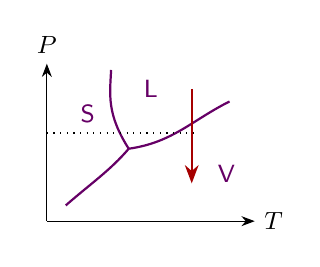
\begin{tikzpicture}[scale=.8]
\draw[->] (0,0)--(3.3,0) node[right]{$T$};\draw[->] (0,0)--(0,2.5) node[above]{$P$};
\draw[pression,thick] (.3,.25)..controls(.7,.6)and(1,.8)..(1.3,1.15)..controls(2,1.25)and(2.3,1.6)..(2.9,1.9);
\draw[pression,thick] (1.3,1.15)..controls(.95,1.7)and(1,2)..(1.02,2.4);\node[pression] at (.65,1.7){S};\node[pression] at (1.65,2.1){L};\node[pression] at (2.85,.75){V};
\draw[dotted] (0,1.4)--(2.4,1.4);\draw[force] (2.3,2.1)--(2.3,.6);
\end{tikzpicture}\end{center}
L'eau passe de l'état liquide à l'état de vapeur : c'est le phénomène de \textbf{cavitation}. Des bulles de vapeur apparaissent et génèrent un bruit.
\end{exemple}
\titr{Expérience réelle}
\begin{center}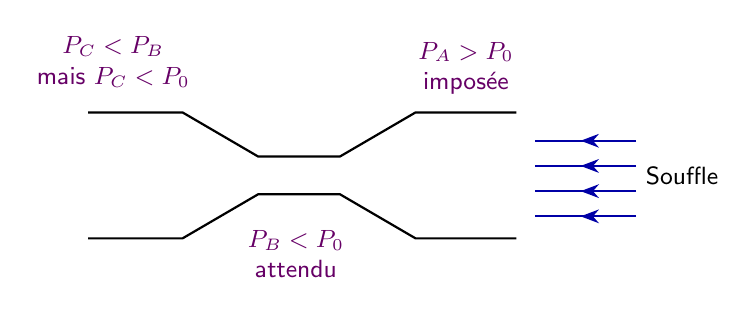
\begin{tikzpicture}[scale=.8]
\venturi
\foreach\y in{-.65,-.25,.15,.55}{\draw[courant] (8.7,\y)--(7.1,\y);}\node[right] at (8.7,0){Souffle};
\node[pression,align=center] at (6,1.7){$P_A>P_0$\\imposée};\node[pression,align=center] at (3.3,-1.25){$P_B<P_0$\\attendu};\node[pression,align=center] at (.4,1.8){$P_C<P_B$\\mais $P_C<P_0$};
\end{tikzpicture}\end{center}
Les pertes énergétiques rendent l'écoulement non parfait : il y a une « perte de charge ».
% Source 21
\subsection{Tube de Pitot}
Le tube de Pitot est aujourd'hui surtout utilisé dans les avions.
Le tube de Pitot date du XVIII\textsuperscript{e} siècle. Son objectif est de mesurer la vitesse de l'écoulement de la Seine, afin de déterminer si $\vec v$ dépend de la profondeur.
\begin{center}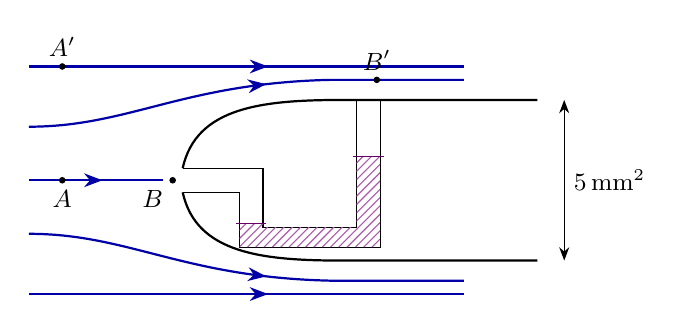
\begin{tikzpicture}[scale=.85]
% Sonde et prises de pression.
\draw[thick] (1.8,.18)..controls(2,1.1)and(3,1.2)..(4.2,1.2)--(7.1,1.2);
\draw[thick] (1.8,-.18)..controls(2,-1.1)and(3,-1.2)..(4.2,-1.2)--(7.1,-1.2);
\draw (1.8,.18)--(3,.18)--(3,-.7)--(4.4,-.7)--(4.4,1.2);
\draw (1.8,-.18)--(2.65,-.18)--(2.65,-1)--(4.75,-1)--(4.75,1.2);
\fill[pattern=north east lines,pattern color=violet!65] (2.65,-.65)--(3,-.65)--(3,-.7)--(4.4,-.7)--(4.4,.35)--(4.75,.35)--(4.75,-1)--(2.65,-1)--cycle;
\draw[pression] (2.6,-.65)--(3.05,-.65) (4.35,.35)--(4.8,.35);
\foreach\sgn in{-1,1}{\draw[courant] (-.5,\sgn*.8)..controls(1,\sgn*.8)and(1.8,\sgn*1.45)..(4,\sgn*1.5)--(6,\sgn*1.5);\draw[courant] (-.5,\sgn*1.7)--(6,\sgn*1.7);}
\draw[courant] (-.5,0)--(1.5,0);\fill(0,0)circle(1.4pt)node[below]{$A$};\fill(1.65,0)circle(1.4pt)node[below left]{$B$};\fill(0,1.7)circle(1.4pt)node[above]{$A'$};\fill(4.7,1.5)circle(1.4pt)node[above]{$B'$};
\draw[<->] (7.5,-1.2)--(7.5,1.2) node[midway,right]{$5\,\mathrm{mm^2}$};
\end{tikzpicture}\end{center}
Le poids est négligé.
Sur la ligne de courant $A\to B$,
\[P_A+\frac12\mu v_A^2=P_B+0,\]
où $B$ est un point d'arrêt. Sur la ligne de courant $A'\to B'$,
\[P_{A'}+\frac12\mu v_{A'}^2=P_{B'}+\frac12\mu v_{B'}^2.\]
% Source 22
Les conditions limites sont $v_A=v_{A'}=v_\infty$ et $P_A=P_{A'}=P_\infty$.
Le tube de Pitot est très petit : le tube de courant a la même section en $A'$ et en $B'$.

Ainsi,
\[v_{A'}=v_{B'}=v_\infty,\qquad\underbrace{P_{A'}}_{P_A}=P_{B'}=P_\infty.\]
\[P_B=P_A+\frac12\mu v_A^2=P_{B'}+\frac12\mu v_\infty^2.\]
\begin{cadre}\[v_\infty=\sqrt{\frac{2(P_B-P_{B'})}\mu}.\]\end{cadre}
Pour $v=40\,\mathrm{m\,s^{-1}}$, on obtient $\Delta P=0{,}01\,\mathrm{bar}$ : cette différence de pression est facile à mesurer.
\subsection{Vidange d'un réservoir}
% Sources 22-23
\begin{center}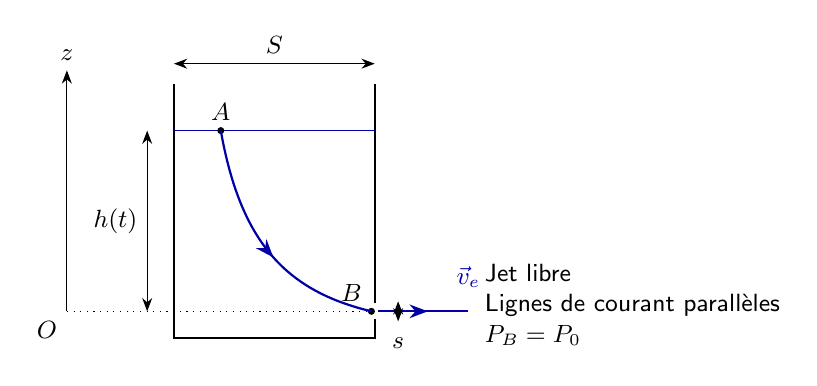
\begin{tikzpicture}[scale=.85]
\draw[->] (-1.6,0)--(-1.6,3.6) node[above]{$z$};\node[below left] at (-1.6,0){$O$};\draw[dotted] (-1.6,0)--(3.3,0);
\draw[thick] (0,3.4)--(0,-.4)--(3,-.4)--(3,-.12) (3,.12)--(3,3.4);\draw[blue!65!black] (0,2.7)--(3,2.7);
\fill(.7,2.7)circle(1.5pt)node[above]{$A$};\fill(2.95,0)circle(1.5pt)node[above left]{$B$};\draw[courant] (.7,2.7)..controls(1,1)and(1.7,.3)..(2.95,0);\draw[courant] (3.05,0)--(4.4,0) node[above=5pt]{$\vec v_e$};
\draw[<->] (-.4,0)--(-.4,2.7) node[midway,left]{$h(t)$};\draw[<->] (0,3.7)--(3,3.7) node[midway,above]{$S$};\draw[<->] (3.35,-.15)--(3.35,.15);\node[below] at (3.35,-.25){$s$};\node[right,align=left] at (4.5,.1){Jet libre\\Lignes de courant parallèles\\$P_B=P_0$};
\end{tikzpicture}\end{center}
Le théorème de Bernoulli sur la ligne de courant $A\to B$ donne
\[P_0+\frac12\mu v_A^2+\mu gh(t)=P_0+\frac12\mu v_e^2+0,\]
\[\frac12\mu v_A^2+\mu gh(t)=\frac12\mu v_e^2.\]
L'écoulement est incompressible : $v_AS=v_es$. D'où
\[\frac12\mu v_e^2\left(\frac sS\right)^2+\mu gh=\frac12\mu v_e^2,\]
\[\mu gh=\frac12\mu v_e^2\left[1-\left(\frac sS\right)^2\right].\]
On choisit $s\ll S$ : on se place dans l'approximation des régimes quasi stationnaires (ARQS), car $h$ décroît très lentement.
\[\left\|\pd{\vec v}t\right\|\ll\|\conv\|.\]
Cela justifie a posteriori les hypothèses permettant d'utiliser le théorème de Bernoulli.
\begin{cadre}\[v_e=\sqrt{2gh(t)}.\]\end{cadre}
% Source 24
\titr{Équation différentielle vérifiée par $h(t)$}
Cf. TD 4, exercice 5.
L'écoulement est incompressible : le débit volumique $D_V$ se conserve à travers toute section du tube de courant global.
\[-S\frac{\dd h}{\dd t}=sv_e=s\sqrt{2gh},\]
\[\frac{\dd h}{\sqrt h}=-\frac{\sqrt{2g}\,s}{S}\,\dd t,\]
\[2\left[\sqrt{h(t)}-\sqrt{h(0)}\right]=-\frac{\sqrt{2g}\,s}{S}t-0.\]
\begin{cadre}\[h(t)=\left(\sqrt{h_0}-\sqrt{\frac g2}\frac sS\,t\right)^2.\]\end{cadre}
Pour calculer le temps de vidange, on prend $t=T$ et $h=0$.
% Source 25
\begin{center}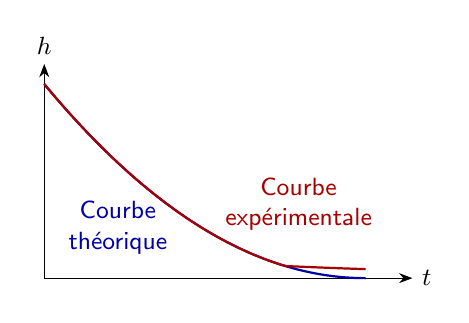
\begin{tikzpicture}[scale=.85]
\draw[->] (0,0)--(5.5,0) node[right]{$t$};\draw[->] (0,0)--(0,3.2) node[above]{$h$};
\draw[blue!65!black,thick,domain=0:4.8,samples=70] plot(\x,{2.9*(1-\x/4.8)^2});
\draw[red!65!black,thick,domain=0:4.8,samples=70] plot(\x,{ifthenelse(\x<3.6,2.9*(1-\x/4.8)^2,.18125*exp(-.25*(\x-3.6)))});
\node[blue!65!black,align=center] at (1.1,.75){Courbe\\théorique};\node[red!65!black,align=center] at (3.8,1.1){Courbe\\expérimentale};
\end{tikzpicture}\end{center}
Un écart apparaît à la fin de la vidange : $h$ est très petit, ses variations ne sont plus négligeables et l'hypothèse de l'ARQS n'est plus vérifiée.
\subsection{Portance et effet Magnus}
\begin{exemple}[breakable]
\textbf{Exercice de cours : aile d'avion}
\begin{center}\cylindre{0}\end{center}
% Source 26
L'écoulement est parfait, incompressible, irrotationnel et stationnaire. On utilise le premier théorème de Bernoulli :
\[P(M)+\frac12\mu v^2=\cste\quad\text{dans tout l'écoulement},\]
\[P(r,\theta,z)=\cste-\frac12\mu v^2.\]
\[\vec F_{\mathrm{pression}}=\iint_\Sigma-P(M)\,\dd^2\vec S=\vec0\quad\text{par symétrie}.\]
\begin{center}\cylindre{1}\end{center}
La portance est nulle pour une aile d'avion cylindrique. Il faut briser la symétrie entre le haut et le bas :
\begin{enumerate}
\item On peut modifier le profil : c'est le cas d'une aile d'avion.
\item On peut mettre le cylindre en rotation : c'est l'effet Magnus.
\end{enumerate}
% Source 27
\titr{1) Modification du profil}\nopagebreak[4]
\begin{center}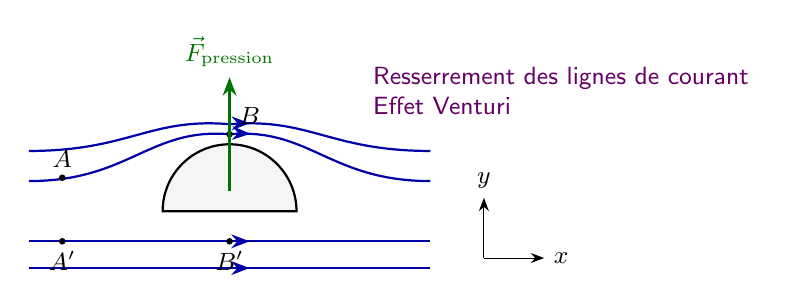
\begin{tikzpicture}[scale=.85]
\draw[thick,fill=gray!8] (-1,0) arc(180:0:1)--cycle;
\foreach\h in{.45,.9}{\draw[courant] (-3,\h)..controls(-1.5,\h)and(-1.2,{1.1+\h/3})..(0,{1+\h/3})..controls(1.2,{1.1+\h/3})and(1.5,\h)..(3,\h);}
\foreach\y in{-.45,-.85}{\draw[courant] (-3,\y)--(3,\y);}\draw[->] (3.8,-.7)--(4.7,-.7) node[right]{$x$};\draw[->] (3.8,-.7)--(3.8,.2) node[above]{$y$};
\fill(-2.5,.5)circle(1.4pt)node[above]{$A$};\fill(-2.5,-.45)circle(1.4pt)node[below]{$A'$};\fill(0,1.15)circle(1.4pt)node[above right]{$B$};\fill(0,-.45)circle(1.4pt)node[below]{$B'$};
\draw[->,green!45!black,thick] (0,.3)--(0,2) node[above]{$\vec F_{\mathrm{pression}}$};
\node[pression,anchor=west,align=left] at (2,1.8){Resserrement des lignes de courant\\Effet Venturi};
\end{tikzpicture}\end{center}
$v_B>v_{B'}$, donc $P_B<P_{B'}$ : la portance est non nulle.
\begin{center}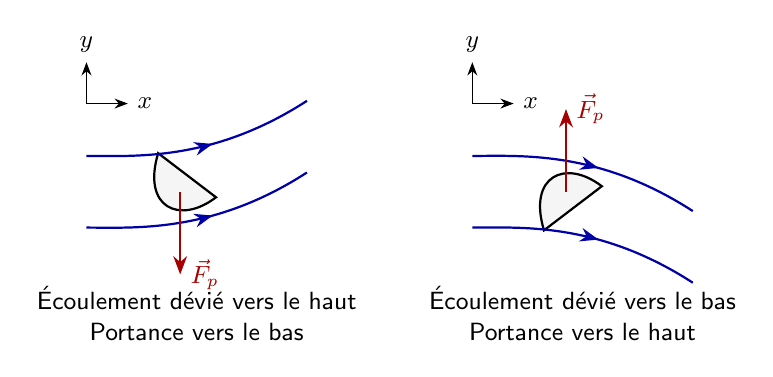
\begin{tikzpicture}[scale=.7]
\begin{scope}[xshift=-3.5cm]\draw[->](-2,1.6)--(-1.25,1.6)node[right]{$x$};\draw[->](-2,1.6)--(-2,2.35)node[above]{$y$};
\draw[thick,fill=gray!8] (-.7,.7)..controls(-1,-.3)and(-.3,-.6)..(.35,-.1)--cycle;
\foreach\y in{-.65,.65}{\draw[courant](-2,\y)..controls(-1.1,\y)and(.3,{\y-.1})..(2,{\y+1});}\draw[force](-.3,0)--(-.3,-1.5)node[right]{$\vec F_p$};\node[align=center]at(0,-2.2){Écoulement dévié vers le haut\\Portance vers le bas};
\end{scope}
\begin{scope}[xshift=3.5cm]\draw[->](-2,1.6)--(-1.25,1.6)node[right]{$x$};\draw[->](-2,1.6)--(-2,2.35)node[above]{$y$};
\draw[thick,fill=gray!8] (-.7,-.7)..controls(-1,.3)and(-.3,.6)..(.35,.1)--cycle;
\foreach\y in{-.65,.65}{\draw[courant](-2,\y)..controls(-1.1,\y)and(.3,{\y+.1})..(2,{\y-1});}\draw[force](-.3,0)--(-.3,1.5)node[right]{$\vec F_p$};\node[align=center]at(0,-2.2){Écoulement dévié vers le bas\\Portance vers le haut};
\end{scope}
\end{tikzpicture}\end{center}
Ces résultats s'interprètent par un bilan des quantités de mouvement.
\textbf{Remarque :} en pratique, il faut étudier le rapport portance-traînée pour optimiser une aile d'avion.
% Sources 27-28
\titr{2) Mise en rotation du cylindre}
\begin{center}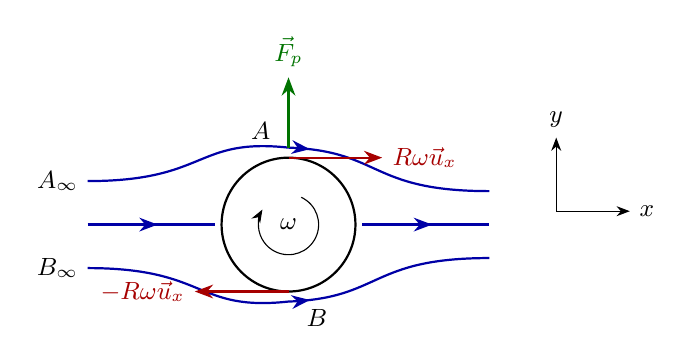
\begin{tikzpicture}[scale=.85]
\draw[thick] (0,0) circle(1);\draw[->] (65:.45) arc(65:-210:.45);\node at (0,0){$\omega$};
\foreach\sgn in{-1,1}{\draw[courant] (-3,\sgn*.65)..controls(-1.2,\sgn*.65)and(-1.4,\sgn*1.3)..(0,\sgn*1.15)..controls(1.4,\sgn*1.1)and(1.2,\sgn*.5)..(3,\sgn*.5);}
\draw[courant](-3,0)--(-1.1,0);\draw[courant](1.1,0)--(3,0);
\node[above left=3pt] at (0,1){$A$};\node[below right=3pt] at (0,-1){$B$};\node[left] at (-3,.65){$A_\infty$};\node[left] at (-3,-.65){$B_\infty$};
\draw[force] (0,1)--(1.4,1) node[right]{$R\omega\ux$};\draw[force] (0,-1)--(-1.4,-1) node[left]{$-R\omega\ux$};
\draw[->,green!45!black,thick] (0,1.15)--(0,2.2) node[above]{$\vec F_p$};\draw[->] (4,.2)--(5.1,.2) node[right]{$x$};\draw[->] (4,.2)--(4,1.3) node[above]{$y$};
\end{tikzpicture}\end{center}
En réalité, l'écoulement est dévié vers le bas. La viscosité dans la couche limite donne $v_A>v_B$.
On applique le théorème de Bernoulli sur $A_\infty\to A$ et $B_\infty\to B$ : $P_A<P_B$.
\begin{center}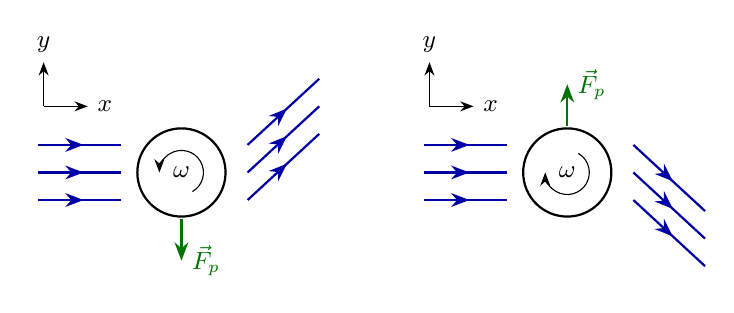
\begin{tikzpicture}[scale=.7]
\foreach\shift/\sgn in{-3.5/-1,3.5/1}{\begin{scope}[xshift=\shift cm]\draw[->](-2.5,1.2)--(-1.7,1.2)node[right]{$x$};\draw[->](-2.5,1.2)--(-2.5,2)node[above]{$y$};
\draw[thick] (0,0) circle(.8);\node at (0,0){$\omega$};
\ifnum\sgn=1\draw[->] (60:.4) arc(60:-180:.4);\else\draw[->] (-60:.4) arc(-60:180:.4);\fi
\foreach\y in{-.5,0,.5}{\draw[courant](-2.6,\y)--(-1.1,\y);\draw[courant](1.2,\y)--(2.5,{\y-\sgn*1.2});}
\draw[->,green!45!black,thick](0,\sgn*.85)--(0,\sgn*1.6)node[right]{$\vec F_p$};
\end{scope}}
\end{tikzpicture}\end{center}
Il s'agit de l'\textbf{\underline{effet Magnus}}.
\end{exemple}
\end{document}